\section[Introdução]{Introdução}

O projeto "Turismo Rural em São Francisco de Paula", idealizado pelos stakeholders Augusto Mussi Alvim e Maurício Schaidhauer, professores da Escola de Negócios da \ac{pucrs}, sob orientação da professora Alessandra Dutra, tem como objetivo principal promover acesso à informação e divulgar rotas e pontos turísticos da cidade por meio de uma aplicação mobile.

A demanda turística no município de São Francisco de Paula tem crescido de forma constante ao longo dos últimos anos. Assim, o aplicativo foi pensado para atender à necessidade de divulgação de informações acerca dos serviços e atrações turísticas disponíveis para visitação, impulsionando o crescimento desse setor da economia. Para atingir tal o objetivo, a aplicação deveria contar com telas de listagem de eventos e atrações turísticas, telas de visualização desses elementos, bem como suas telas de cadastro e a possibilidade de construção de rotas turísticas personalizadas para cada usuário. Para melhor admnistração do aplicativo, também foi adicionada ao escopo, uma tela de login.

Inicialmente, equipe empenhou-se em contruir um ambiente de trabalho marcado por princípios como coolaboração, integração e trabalho em equipe. Isso possibilitou que o andamento do projeto se desse de maneira cordial e, consequentemente, que todos os integrantes recebessem o apoio necessário durante o processo de desenvolvimento.

O primeiro passo para o desenvolvimento do aplicativo foi fabricar um protótipo da aplicação na plataforma figma, com um design limpo, moderno e intuitivo, buscando atrair o público-alvo do projeto, isto é, pessoas com idades pertencentes à todas as faixas-etárias. Além disso, foi feito o design de uma logo e identidade visual próprias para o projeto. 

O processo de desenvolvimento, por sua vez, baseou-se nas escolhas de arquitetura definidas pelo time e no planejamento liderado pelos AGES IV. Para o frontend, o time decidiu pela linguagem Dart, equanto que para o backend foi utilizado Java. Ao final de cada sprint era realizada uma retrospectiva, etapa crucial para entendendimento do que poderia melhorar ao longo do projeto. Além disso, os relatórios de sprint foram essenciais para manter o controle acerca do que foi realizado em cada etapa do desenvolvimento. 

O período de execução do projeto ocorreu durante o primeiro semestre de 2024. O time responsável pela elaboração do aplicativo, formado por estudantes do bacharelado de Engenharia de Software matriculados em diferentes níveis da \ac{pucrs}, encontra-se ilustrado na Figura 1, localizada abaixo.

\begin{figure}[H]
    \centering
    \small
    \caption{Time responsável pelo projeto "Turismo Rural em São Francisco de Paula"}
    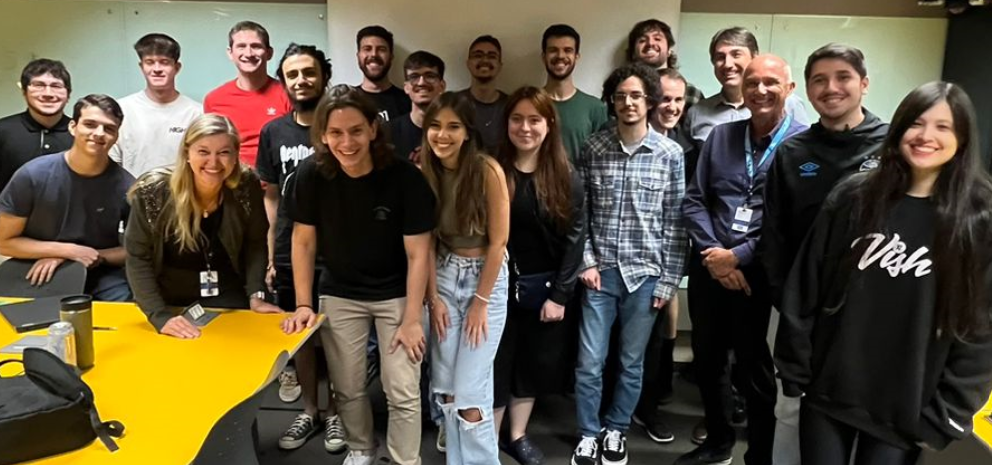
\includegraphics[width=1\linewidth]{conteudo//2 - ages I//conteudo//figures/foto-do-time.png}
    \label{fig:projeto-time-tr}
    \href{https://tools.ages.pucrs.br/o-turismo-rural-em-s-o-francisco-de-paula/wiki/-/wikis/home}{\textit{Fonte: https://tools.ages.pucrs.br/o-turismo-rural-em-s-o-francisco-de-paula/wiki/-/wikis/home}}
\end{figure}